%%%%%%%%%%%%%%%%%%%%%%%%%%%%%%%%%%%%%%%%%%%%%%%%%%%%%%%%%%%%%%%%%%%%%%%%%%%%%%%%
%2345678901234567890123456789012345678901234567890123456789012345678901234567890
%        1         2         3         4         5         6         7         8

\documentclass[letterpaper, 10 pt, conference]{ieeeconf}  % Comment this line out
                                                          % if you need a4paper
%\documentclass[a4paper, 10pt, conference]{ieeeconf}      % Use this line for a4
                                                          % paper

\IEEEoverridecommandlockouts                              % This command is only
                                                          % needed if you want to
                                                          % use the \thanks command
\overrideIEEEmargins
% See the \addtolength command later in the file to balance the column lengths
% on the last page of the document



% The following packages can be found on http:\\www.ctan.org
\usepackage{graphicx} % for pdf, bitmapped graphics files
%\usepackage{epsfig} % for postscript graphics files
%\usepackage{mathptmx} % assumes new font selection scheme installed
%\usepackage{times} % assumes new font selection scheme installed
%\usepackage{amsmath} % assumes amsmath package installed
%\usepackage{amssymb}  % assumes amsmath package installed

\title{\LARGE \bf
A Survey on Software Security in SCADA System
}

\author{ \parbox{3 in}{\centering M Rayhan Ahmed Mithu\\
        % \thanks{*Use the $\backslash$thanks command to put information here}\\
        Department of Computer Science\\
        Tennessee Technological University\\
        Cookeville, TN 38501\\
        {\tt\small mmithu42@students.tntech.edu}}
        % \hspace*{ 0.5 in}
}

% \author{Huibert Kwakernaak$^{1}$ and Pradeep Misra$^{2}$% <-this % stops a space
% \thanks{*This work was not supported by any organization}% <-this % stops a space
% \thanks{$^{1}$H. Kwakernaak is with Faculty of Electrical Engineering, Mathematics and Computer Science,
%         University of Twente, 7500 AE Enschede, The Netherlands
%         {\tt\small h.kwakernaak at papercept.net}}%
% \thanks{$^{2}$P. Misra is with the Department of Electrical Engineering, Wright State University,
%         Dayton, OH 45435, USA
%         {\tt\small p.misra at ieee.org}}%
% }


\begin{document}



\maketitle
\thispagestyle{empty}
\pagestyle{empty}


%%%%%%%%%%%%%%%%%%%%%%%%%%%%%%%%%%%%%%%%%%%%%%%%%%%%%%%%%%%%%%%%%%%%%%%%%%%%%%%%
\begin{abstract}
Internet of things of IoT is the new paradigm in technical advancement. We have moved from smart homes to smart industries. Automation is the priority for most of the manufacturing industries. Supervisory control and data acquisition (SCADA) is one of the most used system in the industrial sector. This system was initially designed for isolated network. SCADA system has recently become part of the bigger network also known as the Internet. This transition has made it possible to manage multiple field sites and connect them through a global network. However, it has also opened up numerous threats and attacking possibilities in this system. Due to the connectivity with the internet, attackers can now directly take control of a filed device which can lead to very destructive attacks. Devices used in SCADA system are resource constrained and cannot perform complex security operations. Lightweight and simple solutions are necessary for this system to protect the information as well as physical infrastructure. In this paper, we discuss the existing work done in this domain and pick out shortcomings of the current work. After detailed analysis of the current work we identify necessary steps required for a complete and secure solution for SCADA system. We also propose a secure architecture for the SCADA system that implements the necessary steps.
\\
\par\noindent Keywords - SCADA, IoT, security, cryptography, Network layer, Application layer, gaps, IDS.

\end{abstract}


%%%%%%%%%%%%%%%%%%%%%%%%%%%%%%%%%%%%%%%%%%%%%%%%%%%%%%%%%%%%%%%%%%%%%%%%%%%%%%%%
\section{INTRODUCTION}
The manufacturing industry is growing fast and with the technological advancement the process is becoming more mechanized and complex. One of the technologies that has grown rapidly in recent years is SCADA system. It plays an important role to manage and control a geographically dispersed industrial network. A typical SCADA system is composed of a control center and large number of field devices. The control center includes a human machine interface (HMI), master terminal unit (MTU) and a database system sometimes called the historian that keeps logs of every action in the system. HMI is the graphical interface of the complete system that presents data to the human operators for monitoring. MTU is responsible to receive information from the filed devices and send it to the control center. It can also occasionally send commands to the field devices. The filed devices are usually a programmable logic controller (PLC) or known as remote terminal units (RTU). RTU communicates with MTU to exchange information about the state of filed devices. At the very lower level there are thousands of sensors and actuators at the filed sites which gathers information from the environment and perform different actions based on commands. With the ever growing demand and growth of the industries,it has become impossible for human to perform in a timely fashion. The growing competition has led to the transition from human to automation which has allowed mass production to be done efficiently and with very little error. More and more businesses are adopting the new technology as a new era of industrialization has begun. Despite most of the earth being covered by water, there is still scarcity of drinkable water in many countries. Water purification is a predominant process for drinkable water supply and automation has been adopted in these infrastructures as well.Energy & Water Development Corp (EAWC) proposed a fully automated system for water purification that will use solar power and other renewable energies when possible \cite{c33}. The system can be controlled remotely over the air with internet. 

Initially SCADA system was designed to automate processes in a single location and it was kept isolated from the outside world.As a result, security was not a big concern for the SCADA system. However, this has changed in recent years and the trend is to connect to the commercial network to create a large interconnected network of multiple field sites. To create this global network SCADA system has now become a part of the public network or the Internet. The consequence of this interconnection is that, SCADA system has now become vulnerable to numerous cyber-attacks and threats. Moreover, The devices used in this system are very low powered and do not have enough resources to handle computationally intensive programs. With very minimum resources, the devices in the SCADA network cannot perform traditional security operations required to protect the system against these new threats. Furthermore, the network traffic and configuration in SCADA system are not compatible with the current standard security mechanisms. Additionally there are back-doors, hard coded security holes and inherent flaws in the firmware of the SCADA devices. SCADA systems are used in critical infrastructures. The consequence of attacks in a SCADA system can be very costly. It could endanger human lives if intended to. Security in SCADA system has become a priority due to all the high risks and new threats.

The recent innovations in the filed of communication and network technology has lead towards a significant advancement in the Internet of Things (IoT). The Internet of Things in industry promises to bring some major changes in the existing system. Although the SCADA systems give operators new capabilities and allow real time control of processes, they also introduce security vulnerabilities. Much work has been done to identify security threats and risks in the IoT in general but relatively less work has been done for the Supervisory control and data acquisition (SCADA) system.

The focus of this paper is to investigate the necessary steps and software techniques used to increase security in SCADA system. Providing a summery of the IoT security issues and challenges in general along with specific finding towards SCADA system. After the in-depth analysis of the work that has been done in this field, we classified different approaches to secure the system. We also identified what are the short comings and possible open research area in this domain. In our analysis of the security issues in SCADA network we found that the use of Intrusion Detection System is immense in securing the network. However, using only the network traffic to monitor anomalies may lead to generation of false positives by the IDS. We believe that, to reduce the number of false positives, additional information is required with the network data. The accuracy of Intrusion Detection System can be improved by adding the relationship of source configuration and generated network traffic. If we can add the specific configuration information related to specific traffic generated in the IDS, it is possible to produce better result and reduce false positives. 

\section{Related Work}
Numerous approaches have been made to reduce false positives in intrusion detection. As discussed in \cite{c30}, the approaches can be divided into two categories, the first approach is to reduce the false positives during the detection process and the second approach is to reduce the false positives after the alert generation. Our approach false into the second category as the IDS verifies the generated alert from network traffic by using the device state information. The process is similar to a feedback mechanism as the IDS uses the device information to cross check the generated network traffic to verify the alert.

Landress \cite{c25} proposed an approach that will utilize a set of artificial intelligence machine learning methods to decrease the number of false positives in anomalous intrusion detection data. This method combines data clustering using the simple K-means algorithm, feature selection that employs the J48 Decision Tree algorithm, and self-organizing maps to effectively reduce false positives.
Pietraszek et al. \cite{c26} presented an approach to reduce false positives by post-processing the alert with data mining and machine learning. They believe that using data mining and machine learning together is the key to solve this issue.
Spathoulas et al. \cite{c27} also proposed a post-processing of alerts to improve the accuracy of intrusion detection. Their filter has three main components, the Neighboring Related Alerts (NRA) component, the High Alert Frequency (HAF) component and the Usual False Positives (UFP) component.
In 2008, Wu and Ye \cite{c31} proposed that the combination of Support Vector Machine (SVM) and Decision Tree algorithm could produce better accuracy in intrusion detection. They used both of these algorithms separately to compare the accuracy, false positive rates for different attacks. Their results show that each algorithm produces better accuracy for certain attack types and hence suggested that combining these two algorithms for overall performance improvement. 
An alert post-processing was done by Siraj et al. in \cite{c32}, where they clustered alerts by discovering feature relationships among sensor data. A causal knowledge based inference technique with fuzzy cognitive modeling was used to cluster the alerts. However, they proposed a single framework for intelligent alert fusion that combines alert prioritization, alert clustering and alert correlation.
\section{Survey Methodology}
This section describes our survey methodology which includes initial study, article selection and the categorization process of the selected articles.

The Internet of Things is a very broad topic with numerous sub-fields that overlaps among each other. Our focus for this survey was on SCADA system which is part of the industrial IoT sector. The technology is evolving and changes all the time. So, to keep our survey up to date with the state of the art, we collected articles published after the year 2000. Furthermore, we prioritized articles from the well-known respected publication sources such as - IEEE, ACM, Springer, Elsevier and conferences related to the topic when looking for articles. 

In our initial study we primarily decided to select article based on two criteria:
\begin{enumerate}
\item The article is specifically related the field of SCADA.
\item Articles cover either software network or device security.

\end{enumerate}

After our initial selection of articles, we started extracting the main ideas and area of focus from these articles. We identified the key attributes of the articles and labeled those into different categories. The categories were drawn out from the common attributes of the articles. The articles were divided into five different categories. Some of the articles fell under more than one category. The categories are described below:

\subsection{Architecture and Layered Security}
The prime focus of the articles in this category is the analysis of the security architecture of the IoT system. The different layers of the architecture such as the application layer and the network layer is described. The security issues in these layers are presented are also presented in the articles.

% \begin{figure}
% \centering
% 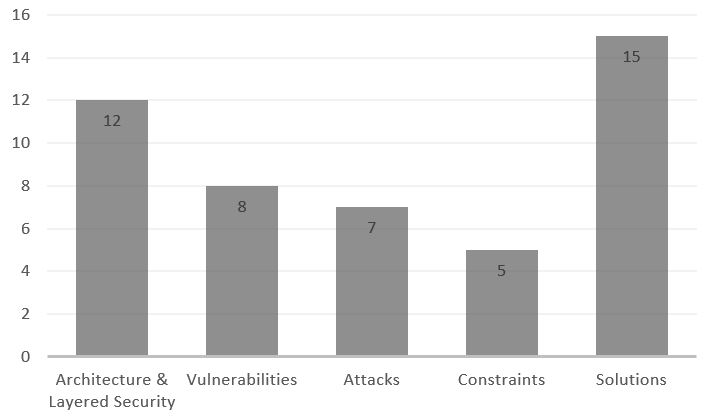
\includegraphics[width=.5\textwidth]{categories}
% \caption{Article categorization}
% \end{figure}

\subsection{Vulnerabilities}
SCADA system has become more vulnerable than ever in recent years. The critical infrastructures controlled by the SCADA system are being targeted and number of attacks are increasing. One of the reason behind this, is the increasing number of vulnerabilities in the system and the communication protocols used in the network. We found that a good number of articles are focused on identifying the vulnerabilities in the system.
\subsection{Attacks}
The articles in this category are more into the read team action then the blue team. A lot of researchers are trying to break into the system and find the security weaknesses is it. Different types of attacks are implemented in testbed architecture and the consequences of the attacks in the system are measured. They analyze how an attacker may try to infiltrate a system which allows other researchers to find a solution for that security weakness.
\subsection{Constraints}
The traditional approaches to protect systems against the cyber-attacks are not always adaptable in the SCADA environment. There are a lot of constraints in the SCADA system which requires a different and much more simpler approach to protect the system from attacking threats. We identified some of the articles that talk about the constraints in the SCADA system and how these constraints affects the security mechanism that are attainable in SCADA environment.
\subsection{Solutions}
There are a large number of new threats and issues discovered in the IoT sector as well as the SCADA environment. Researchers are always coming up with different and new solutions to mitigate these threats and security issues. There are a number of approaches opted by the researches to find solutions to the existing security challenges. We categorized the articles that focuses on providing solutions to these security problems. However, not all the solution used the same approach. We found there are two main broad solutions that are applied in the research.

\begin{itemize}
\renewcommand\labelitemi{--}
\item Hardening security
\item Detection of intrusion
\end{itemize}

After categorizing the articles we studied them and present a survey of the different works that has been done since 2000 in SCADA security. We also look for the gaps, the area where more work needs to be done and future research opportunities in this domain.




\section{Survey}
IoT is at the beginning of a global emergence. Everyday more and more devices and systems are joining the global network. A tremendous amount of work has been done to boost the adoption of IoT in every sector of life starting from home, health to the industry. However, very little efforts have been made towards the security of IoT. Increasing number of exploits and attacks is an indication of the weakness and vulnerability of the IoT security. As the global network is spreading more and more, the risk and consequences of attacks are going to be more devastating. To provide security and prevent the incremental attacks many different solutions are being proposed. The very first step towards a secure network is to identify loopholes in the different layers of the system which requires ample knowledge about the overall architecture of the system. A typical IoT system's architecture consists of three layers, perception layer, network layer and the application layer \cite{c4}\cite{c5}. There are security issues in each of this layers which makes the system vulnerable to a wide range of attacks.
\begin{itemize}
\item \textbf{Perception Layer:} The perception layer is right at the bottom of the architecture consisting of sensors and actuators. This is also called the "Sensors" layer \cite{c4}. Perception layer is responsible for data acquisition by the sensors, data processing and forwarding the collected information to the network layer. This actions are performed by perception node (sensors) and the perception network \cite{c6} respectively. Some of the technologies used in the perception layers are WSNs ( Wireless Sensor Networks), GPS, RFID (Radio Frequency Identification), RSN (RFID Sensor Network) \cite{c4}\cite{c5}\cite{c6}.\\

Even though the layer only performs the data collection and very minimum processing, there still exists security risks in this layer. The authors in \cite{c4} talks about three security issues in the perception layer. First is the strength of wireless signals. Mostly the signals are transmitted between sensor nodes of IoT using wireless technologies whose efficiency can be compromised by disturbing waves. Secondly, the sensor node in IoT devices can be intercepted not only by the owner but also by the attackers because the IoT nodes usually operate in external and outdoor environments, leading to physical attacks on IoT sensors and devices in which an attacker can tamper the hardware components of the device. Third is the inherent nature of network topology which is dynamic as the IoT nodes are often moved around different places. The IoT perception layer mostly consists of sensors and RFIDs, due to which their storage capacity, power consumption, and computation capability are very limited making them susceptible to many kinds of threats and attacks.\\

\item \textbf{Network Layer:} The next layer in the architecture is the network layer. The network layer can be divided into three sub layers based on the functionalities: the access network, core network and the local network. \cite{c6}.

As mentioned before, the network layer of IoT is also susceptible to DoS attacks. Apart from the DoS attacks, the adversary can also attack the confidentiality and privacy at network layer by traffic analysis, eavesdropping, and passive monitoring [1]. These attacks have a high likelihood of occurrence because of the remote access mechanisms and data exchange of devices. The network layer is highly susceptible to Man-in-the-Middle attack [1], which can be followed by eavesdropping. If the keying material of the devices is eavesdropped, the secure communication channel will be completely compromised. The key exchange mechanism in IoT must be secure enough to prevent any intruder from eavesdropping, and then committing identity theft. 
The communication in the IoT is different than that of the Internet because it is not restricted to machine to human. However, the feature of machine-to-machine communication that the IoT introduces has a security issue of Compatibility. The heterogeneity of the network components makes it difficult to use the current network protocols as is, and still produce efficient protection mechanisms. Attackers can also take advantage of the fact that everything is connected in order to gain more information about the users and use this information for future criminal activities [2]. Protecting the network is important in the IoT, but also protecting the objects in the network is equally important. Objects must have the ability to know the state of the network and the ability to protect themselves from any attacks against the network. This can be achieved by having good protocols as well as software that enable objects to respond to any situations and behaviors that can be considered abnormal or may affect their security [7]
\begin{itemize}
\item The access network provided an environment for the perception layer to access the  core network of the system.
\item The core network is responsible for transmitting information from and to different hubs of the IoT infrastructure.
\item The local network is responsible for managing data leakage in the local environment.
\end{itemize}
At this layer, cloud computing platforms, Internet gateways, switching, and routing devices etc. operate by using some of the very recent technologies such as WiFi, LTE, Bluetooth, 3G, Zigbee etc. \\
\item \textbf{Application Layer:} The application layer guarantees the authenticity, integrity, and confidentiality of the data. At this layer, the purpose of IoT or the creation of a smart environment is achieved. this layer at the top of the stack is responsible for delivery of various applications to different users in IoT. The applications can be from different industry verticals such as: manufacturing, logistics, retail, environment, public safety, healthcare, food and drug etc. With the increasing maturity of RFID technology, numerous applications are evolving which will be under the umbrella of IoT.

Since the IoT still does not have global policies and standards that govern the interaction and the development of applications, there are many issues related to application security. Different applications have different authentication mechanisms, which makes integration of all of them very difficult to ensure data privacy and identity authentication. The large amounts of connected devices that share data will cause large overhead on applications that analyze the data, which can have big impact on the availability of the services. 
Another issue that must be considered when designing the applications in IoT is how different users will interact with them, the amount of data that will be revealed, and who will be responsible for managing these applications. The users must have tools to control what data they want to disclose and must be aware of how the data will be used, by whom and when.
\subsection{SCADA network architecture}
Field devices such as sensors and actuators, control devices like a Programmable Logic Controller(PLC) and a control center are the major components of a SCADA network. The network provides communication among the filed devices and control nodes. The control center is usually located in a separate physical part of the factory and typically has advanced computation and communication facilities. Control centers have become very advanced in recent years with Human Machine Interface (HMI) and sometimes have other new servers that provides better management of the entire system. SCADA systems were isolated from the outside network but over the years this has changed as the dispersed network required a centralized control center to manage all the remote sites. As a result, the network was eventually connected to the outside corporate IP based network. This requires a gateway which connects the two different network. Protocols are not same for the SCADA network and the IP network. The gateways are the interface for these two different network and also provides the mechanism to convert communication for the different protocols and enable data transfer between the SCADA network and the corporate network  \cite{c9}.

SCADA networks are unique from the outside networks. The devices used in the filed sites in SCADA networks are mostly very small and are computationally very limited. The typical SCADA network such as a smart grid system is very different from the typical corporate network. The network is geographically extensive than the highly populated corporate office network. Not just the operational conditions but also the physical conditions of a factory where the network is deployed are vastly different from a corporate office environment. The SCADA network is exposed to a lot of strenuous conditions such as dust, radiation and variations in temperature. All of these physical and operational conditions have and effect of the devices. So, the network has to be designed in a way that it can handle all these difficult conditions.

Typical communication in the SCADA network involve a master terminal unit (MTU) and a slave device or Remote Terminal Unit (RTU). PLC is an example of a MTU and the RTU are generally actuators and sensors. The MTU sends commands to the RTU which performs the actions. RTU can also send back message to the MTU. In some cases, communication between peer devices are required and protocols such as PROFIBUS have a hybrid communication model that provides a communication model for master devices \cite{c9}. A lot of other protocols that are used in SCADA system are MODBUS, DNP3. There are different communication pattern in the SCADA network. Typically the messages sent from the filed devices are larges than the command messages sent from the MTU. Prioritization of messages are necessary in the network to make sure the critical messages are sent before any other. Most of the application of SCADA network require real-time communication as it is deployed in critical infrastructures. The network protocol should have features that not only ensure that the critical messages are delivered but that they are delivered within the time constraints.
\begin{figure}
\centering
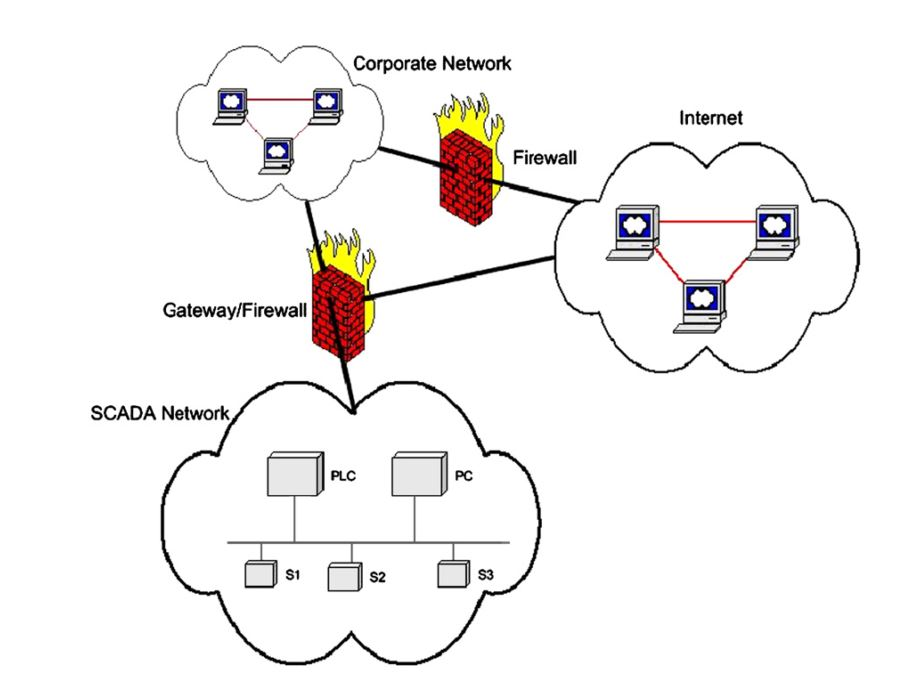
\includegraphics[width=.45\textwidth]{scada_arc}
\caption{Typical SCADA Architecture \cite{c13}}
\end{figure}
\end{itemize}
\subsection{Vulnerabilities}
One of the important aspect of having a secure system is to identify vulnerabilities in the system and come up with solutions against those vulnerabilities. It is mandatory to know what are the weaknesses in the system and how an attacker may use the systems vulnerabilities to break through. This allows to integrate the required security mechanisms to protect the system from the attackers from exploiting these vulnerabilities. 
In recent years the SCADA system has opted to use public networks to provide more interconnections and services among different field sites in multiple locations. This has opened the possibility of new threats and attacks against the SCADA network. The systems are now easily accessible over public network which has introduced a lot of new opportunities but at the same time are susceptible to the traditional attacks in computer networks.
\par
In \cite{c14}, the authors believe that the vulnerabilities in a traditional information technology system have been brought to the SCADA system and the system is now exposed to all the threats that are present in those traditional business systems. Moreover, the technicians involved in SCADA systems are not trained to handle such security problems and lack awareness about all these new threats. Another raising issue is the change of operating systems used in SCADA system. The Linux and Windows operating systems used in SCADA system has flaws and security issues of their own which exposes the system to a new range of operating system level vulnerabilities.
\par
One of the most critical component of the SCADA system is the communication and it is necessary to keep it secure and protected. The recent changes mean that the SCADA system is connected to a wide range of networks. It is not ideal that all the networks will use the same communication protocol. This has led to create vulnerabilities in the communication in SCADA network as the protocols are different. Furthermore, it is mandatory for the SCADA system to communicate in a timely manner as the result of a delay could be devastating sometimes. Due to the nature of broadcasting traffic in some of the older communication protocols, there is a possibility of delay for the SCADA signals in a peak broadcast traffic which is undesirable for critical processes \cite{c15}. The author also mentioned in the paper \cite{c15} that one of the very important vulnerability that still exists is the trust between devices in  a system. However, the problem is slightly addressed by using cryptography in the network which builds trust between networks rather than devices.

Ten et al. proposed a methodology in \cite{c12} to assess vulnerabilities in SCADA system and evaluate the impact of different attacks in the system by exploiting those. The purpose of the methodology is to evaluate consequences of cyber attacks in a power system. The authors' proposed methodology focuses on identifying vulnerability at three different levels: system, scenarios and access points. Two different attack scenario is considered during the  
\subsection{Attacks}
The number of cyber-attacks in to IoT and SCADA system are increasing at an alarming rate. According to \cite{c11} the number of attacks in SCADA system has a significant rise from the 2013 (163,228) to 2014 (675,186), more than doubling in a single year. The result of these attacks are devastating. Critical infrastructure is damaged, valuable information is lost and it can be life threatening in some cases depending on the intention of the attackers. In \cite{c12}, the authors classify the attacks in SCADA system in two categories as the Directed attacks and the Intelligent attacks. Directed attacks are the ones with short term consequences and can be detected from the system behavior. The intelligent attacks are much more sophisticated and do significant damage to the system. This attacks are very well planed and could take about months to even realize by the system administrator.

\begin{itemize}
\item \textbf{Replay Attack:} The replay attacks are the one when an intruder sends back the same request impersonating as the original sender. The effect of this sort of attack may differ according to the data that is being transmitted. The authors provided an example of a water spill gates where signals will be sent using the ZigBee network to open the spill gates. If a request of opening the gate 2 degree is sent more than once than the resulted effect could be damaging as for each request the gates will be opened 2 more degrees.
\item \textbf{Packet Interception: }
One of the communication technology used in SCADA system is the ZigBee and since most of the ZigBee networks do not use encryption at all, it makes Interception of Packets attack possible and feasible for an attacker. It becomes really easy for the attacker to eavesdrop on ZigBee network traffic and abuse the intercepted (probably sensitive) information for their own malicious purposes. The attack can be performed by using KillerBee’s zbdump tool that captures and saves traffic into a capture file.
\item \textbf{Denial of Service (DoS):} The denial of service attack is when the attacker tries to overflow the network with unwanted and malicious requests which overloads the buffer of a particular device. As a result, the legitimate network traffic is dropped due to the overflow and the usual service is hampered.
\end{itemize}
\par
In January 2003, the Slammer worm infected the safety monitoring systems at the Davis-Besse nuclear plant in US. In 2003, two hackers gained access to control technology for the US’s Amundsen-Scott South Pole Station which ran life-support technology for scientists. This attack disabled the safety monitoring system for nearly five hours \cite{c14}.
\par
Operation of more than 100 power plants stopped in the United States on August 14, 2003. The cause of this disaster was a bug in communication systems and about 50 million people living in the US and Canada were affected by this dis- aster and 10 major airports and the New York metro could not serve properly. Another cyber attack on waste management facilities in Queensland, Australia caused a large amount of waste to be discharged into public places. Numerous attacks occur on ICS, another one is the Stuxnet Worm, one of the most sophisticated computer worms thought to be targeted at the Iran Nuclear program and affected more than 100,000 computer systems, have also been reported \cite{c16}.
\subsection{Constraints}
The recent attacks in the industrial control system or cyber-physical has created a major concern in security of these environments. There is a significant difference between the industrial IoT and the traditional IoT. The protocols used in SCADA system are not very similar to the traditional protocols used in commercial network. As a result, the security measures to prevent attacks in the traditional environment cannot be applied in the SCADA system. Not only the protocols but also the devices are not compatible with the existing solutions implemented. The authors in \cite{c19} believe that, it is the constrained devices in the network which are more susceptible to attacks. This highly constrained devices connect with more powerful devices and creates a shared network to exchange information. To protect the information security mechanism such as cryptography is required. However, it is not clear how these resource constraint device will handle such complex algorithms. The authors also suggests, it is necessary to create a lightweight and simple cryptographic solution without reducing the security level for constraint devices in SCADA network.
In \cite{c20}, the authors briefly explains the affects of resource constraint devices in designing security protocols for IoT network. As a result of the low-bandwidth channels used for communication, the security protocol packets might be fragmented. Due to the nature of limited resource and CPU power the strong cryptographic solutions cannot be used in this network. The constraint devices are also vulnerable to attacks that exhausts resources. 
\subsection{Solutions to existing issues}
As the number of new threats and attacks are increasing rapidly the research community is also constantly looking for solutions to these issues. Many different approaches are taken to mitigate these attacks in IoT. We identified some of the techniques that are well known and adopted by the majority of the research community.
\begin{itemize}
\item \textbf{Intrusion Detection System (IDS):} Intrusion detection systems are the reactive measures taken to identify malicious activity and protect the systems from them. There are two different approaches, signature based and anomaly based in IDS to detect unauthorized access. The signature based approach uses rules and policies to decide if any data traffic should be allowed or denied. This approach is easy to implement and can accurately detect well known attacks. However, the signature based IDS will fail to detect any zero day attacks. On the contrary, anomaly based IDS is capable of detecting intrusions based on behavior analysis. This approach is time consuming but can detect attacks that has not been discovered yet. Attackers are always coming up with new and different ways to intrude systems. Defining new rules every time after an attack is discovered is not scalable as some devices may not have enough resources to deal with large rule set. Once trained with a valid dataset the anomaly based IDS builds a model of normal behavior and it can also improve that when new information is learned. 

As the SCADA system has become vulnerable to a host of new attacks, researchers are working towards securing the system with traditional and new approaches. Intrusion detection system is one of the most popular methods for securing communication in SCADA network. Despite having very low powered devices in the SCADA architecture, a large number of research is ongoing to identify intrusion in SCADA system with IDS. However, the approaches to use IDS in SCADA system are not similar in many cases. The authors in \cite{c2} came up with an approach to identify critical states in the SCADA system. The rule based IDS was used in their approach. Critical states of the system were defined and a database of rules for the system was generated. They implemented the IDS on a virtual image of the actual physical system. The virtual image represented the physical devices and the state of the system that was being analyzed. A system representation language was defined called the Industrial State Modeling Language (ISML) \cite{c1}. Even though this language was defined for the MODBUS protocol in SCADA system, it can easily  be extended to support other protocols. Later in 2012 the authors presented an approach to use Critical State-Based Firewall \cite{c3} in SCADA system that could detect critical states to prevent any malicious command or action to be performed.
\item \textbf{Cryptography: }One of the very well known mechanism of protecting information is encryption. The messages transferred between the sender and receiver is encrypted so that, even if the message is intercepted the attacker cannot read the message. There are varying type cryptography such as, using single key to encrypt and decrypt information is known as 'symmetric key encryption' and when the sender and receiver uses different keys to encrypt and decrypt information that is 'asymmetric key encryption'. Sometimes messages are encrypted with hash function as well to provide integrity. There are various cryptographic algorithms which are used to protect the information in transit. Some of the well known algorithms are Advanced encryption standard (AES), Rivest shamir adelman (RSA), Diffie-hellman (DH) and SHA-1/SHA-256. These algorithms are used to provide confidentiality, integrity of the message and source and key management between sender and receiver. 
End-to-end and by-hop are two encryption mechanism that is used when sending encrypted information between two entity. By-hop encryption requires all the nodes to be capable of encrypting and decrypting messages to forward it. On the other hand, end-to-end encryption requires only the sender and receiver node to be capable of performing those actions. By-hop encryption provides better reliability by securing sender and receiver information but increases latency due to encryption mechanism in each node. The end-to-end encryption is faster than this but there is a risk of exposing the source and destination identity if the packet is intercepted \cite{c17}.
Encryption in SCADA systems are not widely used but it has become very important as more and more critical infrastructures are joining the smart network. The data that is transmitted in these infrastructures are very critical and sensitive. Exposure of the data into the wrong hand could prove devastating sometimes. It is necessary to protect the information and using encryption can provide that required security. 
\par One of the most vulnerable communication in SCADA system is the broadcasting of information. It becomes really easy for an attacker to intercept the broadcasted message and use that to gather more information about the network. Encryption of messages can prevent attacks like this. It is also important to understand that the typical cryptographic solutions may not be applicable in SCADA system. As the devices in SCADA environment are not capable of performing complex mathematical operations. Shahzad et al. \cite{c18} proposed a much more optimized cryptography based solution for the DNP3 protocol in SCADA system. They focused on protecting the message broadcasting and proposed a new DNP3 communication stack. The proposed DNP3 stack will use protocol bytes for the encryption mechanism. A cryptography dynamic buffer (CDB) is used to store and keep track of the protocol bytes used for encryption. 
\item \textbf{Hardware:} Whenever IoT comes into our mind we mostly think about the software technology, how it is connecting a large number of devices over the internet and exchanging information. As a result the security issues in the software is all we think about when we try to mitigate attacks in the system. It is expected that majority of the attacks are going to be on the software as it is controlling and managing all these devices. However, most of the devastating attacks are on physical signals during data processing \cite{c10}. 

In \cite{c10}, Teng et al. believe that the security of a system is represented at very lower lever of that system. It is important that security is considered at every level of the system to provide a more secure infrastructure. Most of the devices in an IoT environment or the SCADA environment are equipped with minimum processing capability. The devices are becoming more and more weak in case of computation and becoming much smaller. All of these limitations makes it complicated to provide a software mechanism to secure the system as the devices are not capable of doing most of the intensive work.
According to the authors of \cite{c10}, a solution at the hardware level could prove to be much more successful in this domain. However, there is still a lot to be done in hardware security solutions for IoT. Extensive research is necessary to find a viable solution which can be implemented. The authors present three major drawbacks in the hardware-based solution:
\begin{itemize}
\item The public physical unclonable function (PPUF) is required
\item The PUF is unstable with respect to operational and environmental conditions due to device aging
\item The first generation of PUFs are analog and therefore cannot be integrated into the digital design
\end{itemize}
\end{itemize}






\section{Identified Gap}
There is a large number of researches towards finding security issues in the SCADA network and addressing the issues are being conducted around the globe. Different approaches are being implemented when mitigating security threats and vulnerabilities. Most of the techniques focuses on analyzing the network traffic and recognizing abnormalities in the network traffic. In our literature, we found that there hasn't been enough effort to collaborate network packets along with device states to identify intrusion and malicious activity. This is a very unique approach to verify information received from network packets. The state of the device at any moment must be in sync with the information it sends back to the control center. One of the most used security measure is the intrusion detection system. The IDS uses network packets to find anomalies in the traffic and generate alerts, which often times produces false positives. However, using the device state information the number of false positives can be reduced by validating the generated alert. 
\par
In the literature we found that people are working to solve these steps separately but not as a whole. Some work has been done in defining states of the device and identifying critical states of SCADA system \cite{c3}. It is also suggested that the intrusion detection process and computation will be too much to handle for the SCADA system devices. Which has led to a number of research where a new layer also known as the fog technology that lies in between the control center and the filed devices to filter through packets and look for malicious activity. The devices in this layer have better computational power than field devices. Even though there has been some work in state analysis of SCADA devices to detect malicious activity or command, there has not been enough effort to combine this information with the network traffic and validate the result of a intrusion detection system from the network packets. Our survey leads to three major open research questions that must be answered. these are:
\begin{enumerate}
    \item \textbf{How can we describe, gather and detect the source configuration ?}\par
    By analyzing the configuration of a device, it is possible to infer what actions are triggered when a particular network packet is generated. To analyze the configuration file, it is necessary to normalize the data to detect relationship with network data. Furthermore, the important objects and their values can be inferred from the configuration of the device. We must consider the security of the configuration files as well. It is necessary to make sure that the configuration file is not tampered with.\par
    Hadeli et al \cite{c21} proposed a system that takes the system description file and analyzes it to generate security configurations to detect malicious and missing traffic in the network. After analyzing the system description or configuration file it creates communication model of the network. Furthermore, it also generates Snort rules to detect missing traffic that are not observed in the network.
    Oman et al. \cite{c22} proposed a mechanism to automatically collect the device settings regularly form SCADA devices and compare the settings with previous settings to make sure no unauthorized changes have been made in the device.

    \item \textbf{ How can we quantify the relationship between the source configuration and generated traffic data?}\par
    After identifying the important objects that correlate with the network traffic, the next thing is to quantify this relationship in a way that can be used in the IDS to associate with certain network traffic. Providing specific relationship between the device configuration and network data can improve the accuracy of the IDS. Figure 1 shows the improvement when a value was added to specify a certain network packet in the network data. The accuracy to identify that network data significantly improved.
    \item \textbf{ Which algorithm will work best for the SCADA system?}\par
    There are different machine learning algorithms that can be used in the intrusion detection system. However, not all the algorithms will work for SCADA system due to the resource constraints. It is our next job to identify the algorithms that works for the SCADA system and how the algorithms react to the added information. Many researchers have proposed different approaches to use machine learning in SCADA network for anomaly detection. Magaras et al. proposed an intrusion detection system that uses OCSVM (one class support vector machine) detect malicious activity in the SCADA network. OCSVM is a unique classifies that requires only one source of data from a single class which makes it ideal to be used in SCADA system.

\end{enumerate}
\section{Proposed Architecture}
After identifying the five steps that we believe is required to achieve a secure SCADA system, we focused on how to achieve these steps in a system. Implementing these five steps will require some changes in the current architecture of the SCADA system. We propose an architecture for a SCADA system that can overcome the current security short comings by implementing all the steps mentioned earlier and improve the security of the system. The architecture has three major system components that is focused on completing the steps. Each step will which are:
\begin{enumerate}
\item Off-line Tools
\item SCADA components
\item Detection Process
\subsection{Off-line Tools}
This system component of the architecture is responsible to identify important information about the state of the device and the location of those state information on the device. We call this component the off-line tools as these will be executed when the SCADA system is not running real time. We propose three modules for this component. 
\par The first module is called the \textit{\textbf{Image Mapping Module}}, this module is responsible for identifying the important information to represent the device state and gather those information.
\par The second module will be the \textit{\textbf{Golden Image Module}} which will use the information collected by the image mapping module and create the golden image of the device system which is considered to be safe and standard. \par The third module in this component is the \textit{\textbf{Training Module}}, this module will be used to help the detection process of any malicious activity. The training module will be fed data collected from the SCADA environment with different device state and and mapped with the golden image to learn more about malicious states of the device. This information will be provided to the the detection process to identify a critical or bad state of the device more accurately and fast.
\end{enumerate}
\begin{figure}
\centering
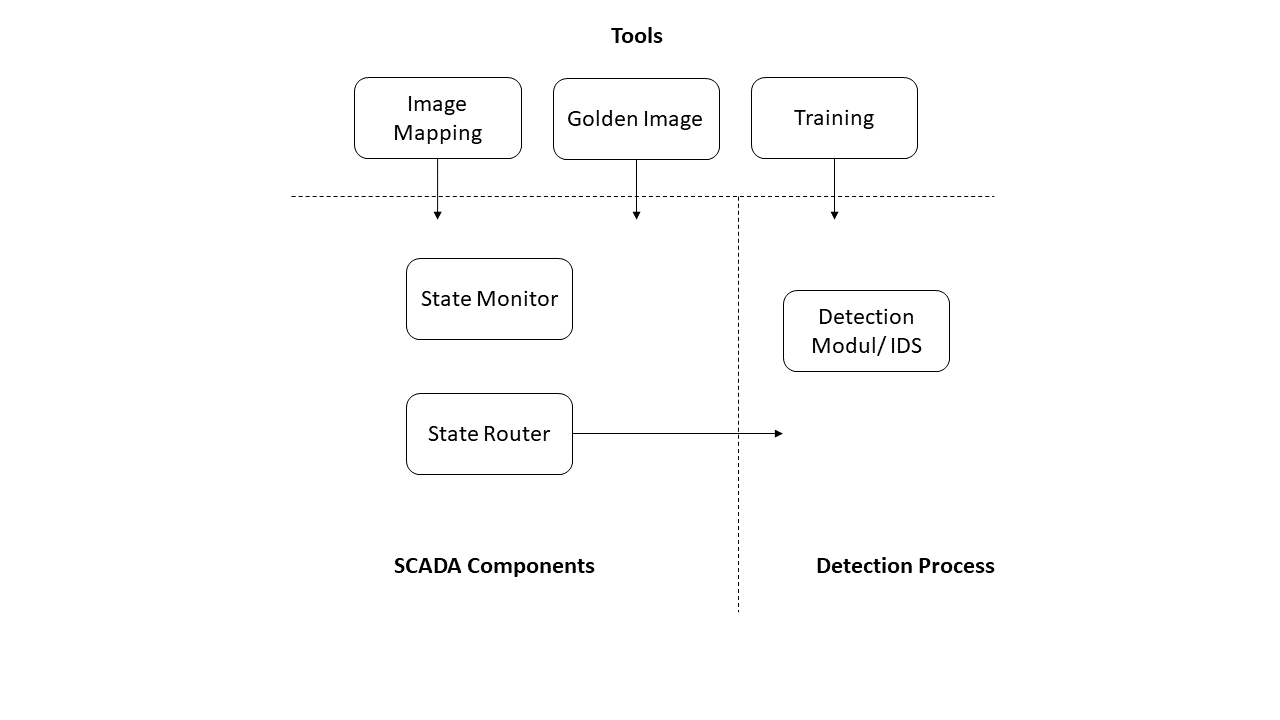
\includegraphics[width=.4\textwidth]{architecture}
\caption{Proposed Architecture}
\end{figure}
\subsection{SCADA Components}
The second component of our architecture is the SCADA components. This component of the system will monitor system states real time and transfer the state information to the detection process. Two modules are required to execute these actions. The first module is the \textit{\textbf{State Monitor}} and the other module is called \textit{\textbf{State Router}}.
\par The state monitor module is responsible for real time monitoring of the device state. The information collected by the image mapping module in the off-line tools component is used in this module to gather the important sate information from the device. State monitor module will have prior knowledge of what information are necessary to represent the state and where the information are kept in the device. 
\par The device state information collected by the state monitor module will be transferred by the state router module to the node that is computationally more resourceful. This node can perform security analysis to identify if the device is compromised.
\subsection{Detection Process}
Detection process is the most important component of the secure architecture. This process is responsible for intrusion detection in the SCADA environment. Typical intrusion detection system (IDS) uses the network packets to analyze the traffic and generate alert in case of any abnormal activity in the network. However, in SCADA environment, it is not necessary that an abnormal network behavior will always be the reason for intrusion. Often times a series of valid commands can lead to a critical situation in the SCADA environment that will cause serious damage to the infrastructure. The IDS will not generate any alert in that situation as the network traffic will not look suspicious or abnormal.
\par The intrusion detection system in this component uses the information gathered by the training module in the off-line tools component to learn about device state. The IDS also receives real time information from the state router and performs analysis to detect compromised device. The information from the state router is also used to improve the IDS detection engine based on the accuracy of intrusion detection. The main idea in the detection process is to provide additional information to the IDS along with the network packets to improve the detection method. The device state information will help the IDS to verify any alert generated from analyzing the network traffic of the SCADA system. 
\section{Future Directions}
Security issues in SCADA system are increasing rapidly. SCADA system has become vulnerable to a new range of attacks after joining the internet. There are numerous work done in securing the system. Different solutions are being proposed and new solutions are still being investigated. However, there has not been any complete solution for a secure SCADA system. As we have categorized some of the possible research directions for securing SCADA system, we want to pursue a research towards one of the gaps. We are going to see if the state of a SCADA device can be correlated with the network packets generated for that particular state. The idea is to help the IDS learn from network packets about the state of the device and use that to trigger alert of any critical or unknown state. After identifying the key steps required to achieve a secure system and proposing an architecture, our future goal is to come up with a proof of concept that the state information will improve intrusion detection system.
\
   
\section{CONCLUSIONS}
Smart technologies have made our life a lot easier than it was a decade ago. Almost everything around us are turning into smart technology recently. This rapid growth of technology has had an effect on industrial revolution as well. Smart industry is not just an idea anymore. Manufacturing industries are moving towards total automation. This transition has created a global network of smart industries. SCADAD system is one of the most widely used technology in industry. It is also joining the smart network and as a result of that, the system has become vulnerable to new threats. SCADA system was initially designed to be isolated from the outside network. Therefore, it is not capable of handling complex security mechanism that are required to protect the system form the new threats and attacks. Even though, there are a number of solutions proposed for SCADA system, an ideal solution is still missing. It is necessary to come up with a complete and secure architecture for SCADA system so that all the valuable information can be protected. In this paper, gaps in current research in secure SCADA system and necessary steps and architecture to achieve a complete solution is presented.
\addtolength{\textheight}{-12cm}   % This command serves to balance the column lengths
                                  % on the last page of the document manually. It shortens
                                  % the textheight of the last page by a suitable amount.
                                  % This command does not take effect until the next page
                                  % so it should come on the page before the last. Make
                                  % sure that you do not shorten the textheight too much.

%%%%%%%%%%%%%%%%%%%%%%%%%%%%%%%%%%%%%%%%%%%%%%%%%%%%%%%%%%%%%%%%%%%%%%%%%%%%%%%%



%%%%%%%%%%%%%%%%%%%%%%%%%%%%%%%%%%%%%%%%%%%%%%%%%%%%%%%%%%%%%%%%%%%%%%%%%%%%%%%%



%%%%%%%%%%%%%%%%%%%%%%%%%%%%%%%%%%%%%%%%%%%%%%%%%%%%%%%%%%%%%%%%%%%%%%%%%%%%%%%%




%%%%%%%%%%%%%%%%%%%%%%%%%%%%%%%%%%%%%%%%%%%%%%%%%%%%%%%%%%%%%%%%%%%%%%%%%%%%%%%%



\begin{thebibliography}{99}
\bibitem{c1} Nai Fovino, I., Coletta, A., Carcano, A., \& Masera, M. (2012). Critical state-based filtering system for securing SCADA network protocols. IEEE Transactions on Industrial Electronics, 59(10), 3943–3950. https://doi.org/10.1109/TIE.2011.2181132
\bibitem{c2} Fovino, I. N., Carcano, A., De Lacheze Murel, T., Trombetta, A., \& Masera, M. (2010). Modbus/DNP3 state-based intrusion detection system. Proceedings - International Conference on Advanced Information Networking and Applications, AINA, 729–736.https://doi.org/10.1109/AINA.2010.86.
\bibitem{c3} Carcano, A., Coletta, A., Guglielmi, M., Masera, M., Nai Fovino, I., \& Trombetta, A. (2011). A multidimensional critical state analysis for detecting intrusions in SCADA systems. IEEE Transactions on Industrial Informatics, 7(2), 179–186. https://doi.org/10.1109/TII.2010.2099234
\bibitem{c4} Bandyopadhyay, D., \& Sen, J. (2011). Internet of things: Applications and challenges in technology and standardization. In Wireless Personal Communications (Vol. 58, pp. 49–69). https://doi.org/10.1007/s11277-011-0288-5
\bibitem{c5} Mahmoud, R., Yousuf, T., Aloul, F., \& Zualkernan, I. (2016). Internet of things (IoT) security: Current status, challenges and prospective measures. In 2015 10th International Conference for Internet Technology and Secured Transactions, ICITST 2015. https://doi.org/10.1109/ICITST.2015.7412116
\bibitem{c6}Jing, Q., Vasilakos, A. V., Wan, J., Lu, J., \& Qiu, D. (2014). Security of the Internet of Things: perspectives and challenges. Wireless Networks, 20(8), 2481–2501. https://doi.org/10.1007/s11276-014-0761-7
\bibitem{c7} Chandia, R., Gonzalez, J., Kilpatrick, T., Papa, M., \& Shenoi, S. (2007). Security Strategies for SCADA Networks. In Critical Infrastructure Protection (pp. 117–131). Boston, MA: Springer US. https://doi.org/10.1007/978-0-387-75462-8\_9
\bibitem{c8} Hentea, M. (2008). Improving security for SCADA control systems. Interdisciplinary Journal of Information, Knowledge, and Management, 3, 73–86. Retrieved from http://ijikm.org/Volume3/IJIKMv3p073-086Hentea361.pdf
\bibitem{c9} Igure, V. M., Laughter, S. A., \& Williams, R. D. (2006). Security issues in SCADA networks. Computers and Security, 25(7), 498–506. https://doi.org/10.1016/j.cose.2006.03.001
\bibitem{c10}Xu, T., Wendt, J. B., \& Potkonjak, M. (2014). Security of IoT systems: Design challenges and opportunities. Proceedings of the 2014 IEEE/ACM International Conference on Computer-Aided Design, 417–423. Retrieved from http://isisell.com/freeupload/34783security of iot systems design challenges and opportunities.pdf
\bibitem{c11}http://www.datacenterdynamics.com/content-tracks/security-risk/scada-cyber-attacks-double-over-the-last-year/93738.fullarticle
\bibitem{c12}Ten, C. W., Liu, C. C., \& Manimaran, G. (2008). Vulnerability assessment of cybersecurity for SCADA systems. IEEE Transactions on Power Systems, 23(4), 1836–1846. https://doi.org/10.1109/TPWRS.2008.2002298
\bibitem{c13}Coates, G. M., Hopkinson, K. M., Graham, S. R., \& Kurkowski, S. H. (2010). A trust system architecture for SCADA network security. IEEE Transactions on Power Delivery, 25(1), 158–169. https://doi.org/10.1109/TPWRD.2009.2034830
\bibitem{c14}Hentea, M. (2008). Improving security for SCADA control systems. Interdisciplinary Journal of Information, Knowledge, and Management, 3, 73–86. Retrieved from http://ijikm.org/Volume3/IJIKMv3p073-086Hentea361.pdf
\bibitem{c15}T. Brown, "Security in SCADA systems: how to handle the growing menace to process automation," Computing \& Control Engineering Journal, vol. 16, (3), pp. 42-47, 2005.
\bibitem{c16}Yılmaz, E. N., \& Gönen, S. (2018). Attack detection/prevention system against cyber attack in industrial control systems. Computers and Security. https://doi.org/10.1016/j.cose.2018.04.004
\bibitem{c17}Suo, H., Wan, J., Zou, C., \& Liu, J. (2012). Security in the internet of things: A review. In Proceedings - 2012 International Conference on Computer Science and Electronics Engineering, ICCSEE 2012 (Vol. 3, pp. 648–651). https://doi.org/10.1109/ICCSEE.2012.373
\bibitem{c18}Shahzad, A., Lee, M., Lee, C., Xiong, N., Kim, S., Lee, Y.-K., … Jeong, G. (2016). The protocol design and New approach for SCADA security enhancement during sensors broadcasting system. Multimed Tools Appl, 75, 14641–14668. https://doi.org/10.1007/s11042-015-3050-2
\bibitem{c19}Roman, R., Najera, P., \& Lopez, J. (2011). Securing the Internet of things. Computer, 44(9), 51–58. https://doi.org/10.1109/MC.2011.291
\bibitem{c20}T. Heer, O. Garcia-Morchon, R. Hummen, S. L. Keoh, S. S. Kumar, and K. Wehrle, “Security challenges in the IP-based Internet of Things,” Wirel. Pers. Commun., vol. 61, no. 3, pp. 527–542, Dec. 2011.
\bibitem{c21}Hadeli, H., Schierholz, R., Braendle, M., \& Tuduce, C. (2009). Generating configuration for missing traffic detector and security measures in industrial control systems based on the system description files. 2009 IEEE Conference on Technologies for Homeland Security, HST 2009, 503–510. https://doi.org/10.1109/THS.2009.5168079
\bibitem{c22}Oman, P., \& Phillips, M. (2007). Intrusion detection and event monitoring in SCADA networks. IFIP International Federation for Information Processing, 253, 161–173. https://doi.org/10.1007/978-0-387-75462-8\_12
\bibitem{c23}Maglaras, L. A., \& Jiang, J. (2014). Intrusion detection in SCADA systems using machine learning techniques. Proceedings of 2014 Science and Information Conference, SAI 2014, 626–631. https://doi.org/10.1109/SAI.2014.6918252
\bibitem{c24}Beaver, J. M., Borges-Hink, R. C., \& Buckner, M. A. (2013). An evaluation of machine learning methods to detect malicious SCADA communications. Proceedings - 2013 12th International Conference on Machine Learning and Applications, ICMLA 2013, 2, 54–59. https://doi.org/10.1109/ICMLA.2013.105
\bibitem{c25}Landress, A. D. (2016). A hybrid approach to reducing the false positive rate in unsupervised machine learning intrusion detection. In Conference Proceedings - IEEE SOUTHEASTCON (Vol. 2016–July). https://doi.org/10.1109/SECON.2016.7506773
\bibitem{c26}Pietraszek, T. (2003). Recent Advances in Intrusion Detection. International Workshop on Recent Advances in Intrusion Detection, 2820, 102–124. https://doi.org/10.1007/b13476
\bibitem{c27}Spathoulas, G. P., & Katsikas, S. K. (2010). Reducing false positives in intrusion detection systems. Computers and Security, 29(1), 35–44. https://doi.org/10.1016/j.cose.2009.07.008
\bibitem{c28}Lin, Y. D., Lai, Y. C., Ho, C. Y., & Tai, W. H. (2013). Creditability-based weighted voting for reducing false positives and negatives in intrusion detection. Computers and Security, 39(PART B), 460–474. https://doi.org/10.1016/j.cose.2013.09.010
\bibitem{c29}Pietraszek, T., & Tanner, A. (2005). Data mining and machine learning - Towards reducing false positives in intrusion detection. Information Security Technical Report, 10(3), 169–183. https://doi.org/10.1016/j.istr.2005.07.001
\bibitem{c30}Mokarian, A., Faraahi, A., & Delavar, A. G. (2013). False Positives Reduction Techniques in Intrusion Detection Systems-A Review. International Journal of Computer Science and Network Security, 13(10), 128–134. https://doi.org/10.1002/fedr.200511077
\bibitem{c31}Wu, S. Y., & Yen, E. (2009). Data mining-based intrusion detectors. Expert Systems with Applications, 36(3 PART 1), 5605–5612. https://doi.org/10.1016/j.eswa.2008.06.138
\bibitem{c32}Siraj, A., & Vaughn, R. B. (2005). Multi-level alert clustering for intrusion detection sensor data. Annual Conference of the North American Fuzzy Information Processing Society - NAFIPS, 2005, 748–753. https://doi.org/10.1109/NAFIPS.2005.1548632
\bibitem{c33}SOLAR POWERED WATER PURIFICATION SYSTEM, Swiss Water Tech Research & Development SA, viewed 19/9/19, http://swisswatertech.com/Water-Purification-System.html
\end{thebibliography}



\end{document}
